% !TeX root = ../paper.tex
\section{Behavioral Intervention Diagnosis Protocol}
\label{appendix:behavior-diagnostics}

\subsection{Condition Construction and Instance Pairing}

We evaluate $\pi_{0.5}$, GR00T N1.6, and StarVLA under four conditions:
ORI, Semantic (Sem), Visual Prompt (Vis), and Control (Con). ORI retains the original task
instruction and scene to
measure basic task execution. Semantic keeps the scene and task context
executable while changing the object, local action, target relation, or
holding/termination requirement. Vis changes object or target layout,
or adds a circle, point, region, or trajectory in the image as the visual
target. Control starts from an intermediate state in which the robot holds
the object and replaces the target or subsequent process requirement.
The initial held state in Control is not counted as a new object
selection.

The three models use the same instances, environment initializations, and
intervention commands. Each model is evaluated on 100 instances per
condition, for 1,200 rollouts in total. Semantic commands cover phase
sub-tasks, atomic motions, object roles, spatial relations, and holding or
termination requirements. Visual prompts are synchronized with the current
object or target region, and Control commands are applied only to
physically executable intermediate states. For each rollout, we record the original
task, initialization, intervention command, and applicable evaluation conditions.

\subsection{Behavioral Metrics}

We report three binary metrics:

\begin{itemize}
\item
  \textbf{Target-object selection rate}: the specified object is correctly
  grasped at least once during execution. This metric is not applicable
  to Control, which starts with an object already held.
\item
  \textbf{Target-position attainment rate}: the manipulated object reaches
  the position, region, or target relation specified by the current
  instruction at least once.
\item
  \textbf{Instruction-completion rate}: all applicable relational,
  sequential, release, holding, and termination requirements are
  satisfied.
\end{itemize}

Correct object selection or transient target attainment does not imply
complete execution. These metrics decompose the behavioral chain and do
not replace the LIBERO-SMART trajectory contract or define a ranking
across architectures.

\subsection{Trajectory Review}

Behavior is judged jointly from state trajectories, action trajectories,
and task conditions. Representative rollouts are reviewed frame by frame
to determine whether the correct object was selected, whether the target
changed with the current condition, whether the obsolete task continued,
and whether unnecessary actions occurred after a local goal was reached.
The main recurring failure patterns are summarized in
Table~\ref{tab:behavior-failure-patterns} and illustrated in
Figure~\ref{fig:behavior-examples}. The complete quantitative
metrics are reported in Appendix~\ref{appendix:representation-diagnostics},
Table~\ref{tab:diagnostics}.

\subsection{Behavioral Results and Failure Patterns}
\label{behavioral-diagnosis}

All three models correctly select the object and reach the original target under ORI, with
complete-task success rates of 96--99\%. Under Sem, target-object selection remains at 79--88\%, but
target-position attainment drops to 3--11\%, and instruction completion falls to only 1--6\%.
Correctly identifying and grasping the object therefore does not ensure that the subsequent
execution satisfies the specified local action, target relation, or holding and termination
requirements.

Under Vis, target-object selection remains at 72--83\%, while target-position attainment is only
3--14\% and instruction completion is only 2--5\%. Under Con, target-position attainment and
instruction completion range from 6\% to 25\%, despite starting from a physically executable state
with the object already held. These results distinguish object selection, target-position
attainment, and complete instruction execution: success at an earlier part of the behavior does not
guarantee that subsequent actions satisfy the current instruction. Table~\ref{tab:diagnostics}
reports the full results.

% !TeX root = ../paper.tex
\begin{center}
\setlength{\belowcaptionskip}{\baselineskip}
\captionof{table}{Recurring behavior patterns observed in trajectory review.}
\label{tab:behavior-failure-patterns}
\normalsize
\setlength{\tabcolsep}{3.5pt}
\begin{tabular}{@{}lll@{}}
\toprule
Pattern & Observable behavior & Capability gap \\
\midrule
Target carryover & Correct grasp, original target retained & Target rebinding \\
Visual-target decoupling & Placement not bound to the visual cue & Visual-prompt grounding \\
Command inertia & Old sequence continues after update & Mid-execution correction \\
Unrequested continuation & Grasp followed by unwanted placement & Termination and holding \\
\bottomrule
\end{tabular}
\end{center}
%

Figure~\ref{fig:behavior-examples} compares $\pi_{0.5}$ and SmartVLA on four
diagnostic tasks, highlighting whether execution follows the instructed
object--target relation, visual prompt, updated destination, or holding
requirement.

% !TeX root = ../paper.tex
\begin{figure}[!htbp]
  \centering
  \setlength{\parskip}{0pt}
  \setlength{\abovecaptionskip}{\baselineskip}
  \setlength{\belowcaptionskip}{0pt}
  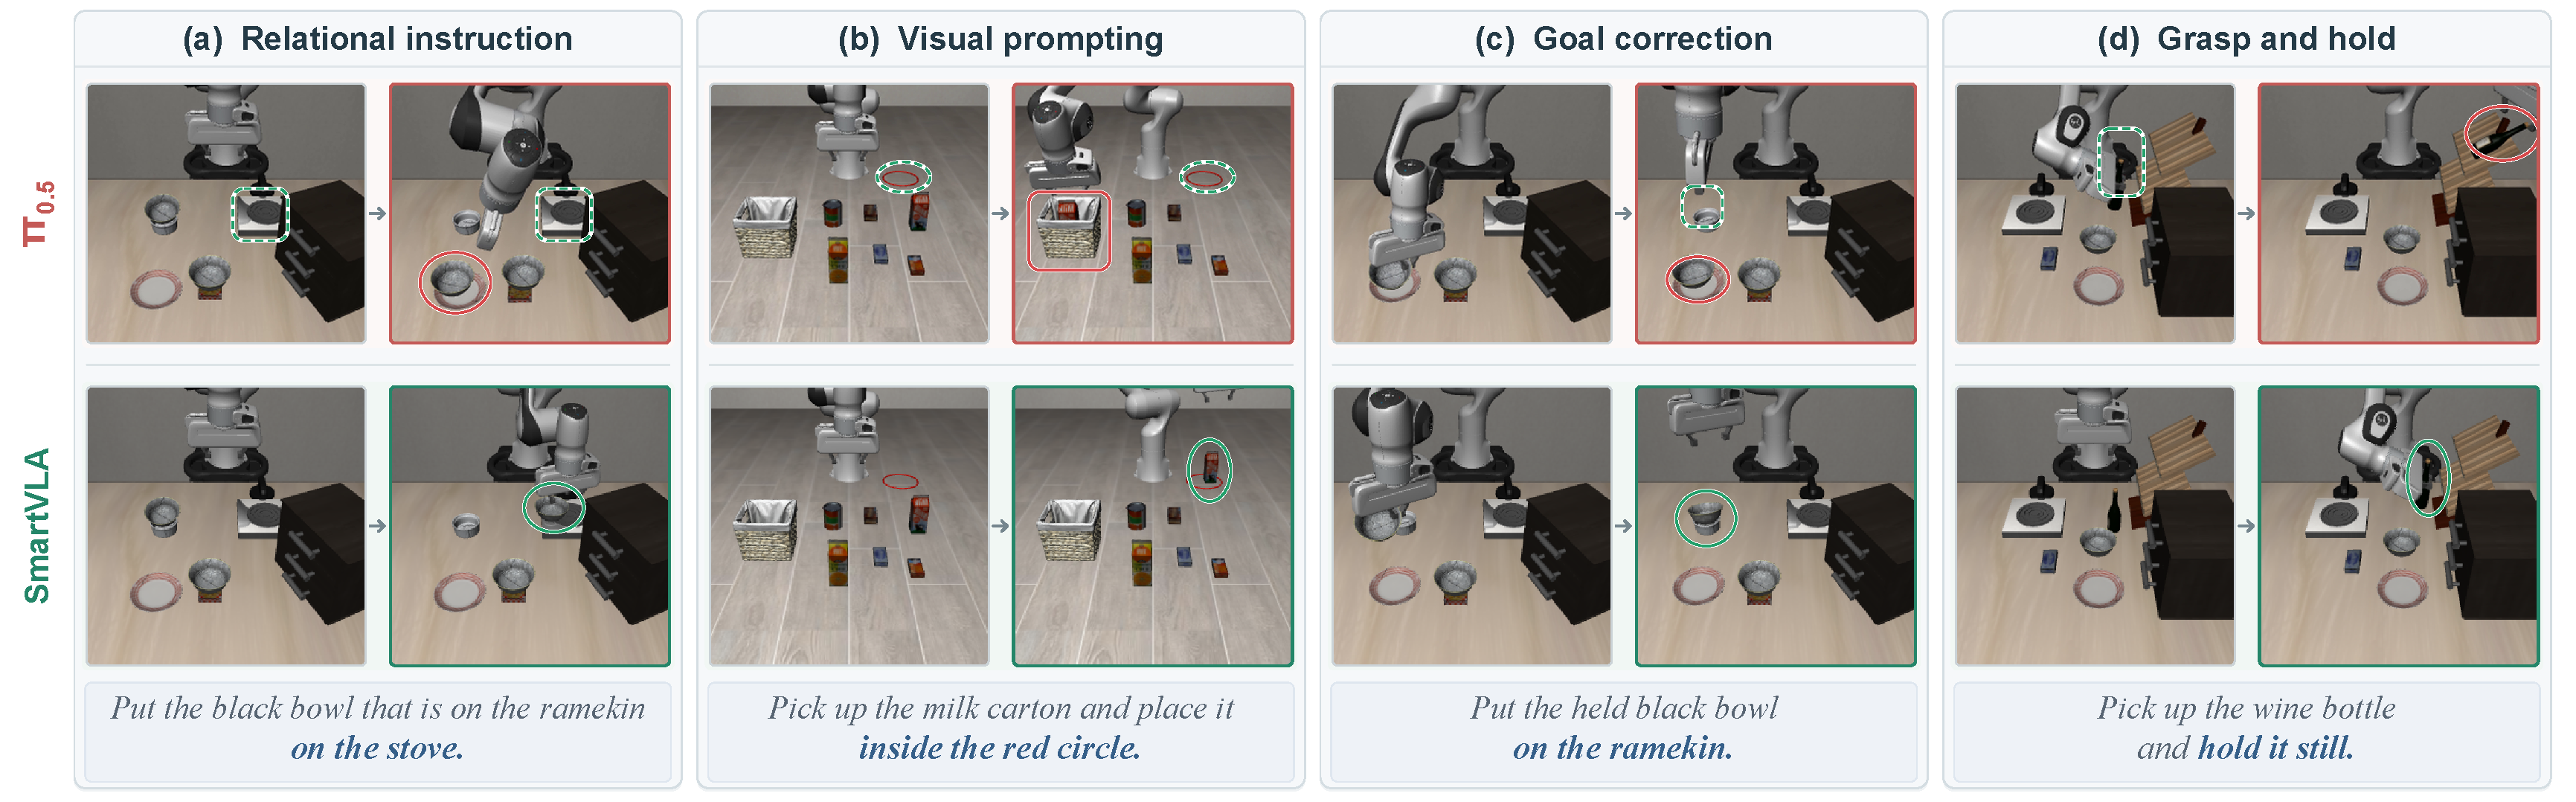
\includegraphics[width=\textwidth]{figures/fig_behavior_comparison_v5.pdf}\par\nointerlineskip
  \caption{Qualitative comparison of $\pi_{0.5}$ (upper row) and SmartVLA
  (lower row) under the same diagnostic instructions. Instructions appear
  below each column; paired frames progress from left to right.
  (a) Relational instruction: placing the specified bowl on the stove
  rather than the plate. (b) Visual prompting: placing the milk inside the
  red circle rather than the basket. (c) Goal correction: redirecting the
  held bowl to the ramekin rather than the plate. (d) Grasp and hold:
  keeping the wine bottle grasped rather than continuing to place it on
  the rack. $\pi_{0.5}$ continues toward an unintended placement target, whereas
  SmartVLA follows the requested destination or holding condition.}
  \label{fig:behavior-examples}
  \label{fig:behavior-success-examples}
\end{figure}
%

